\chapter{Kirjautumismenetelmien turvallisuus\label{Turvallisuus}}

Tässä luvussa esitellään kirjautumismenetelmien turvallisuutta. Luvussa perehdytään kirjautumismenetelmien turvallisuusongelmia ja tutkitaan esimerkkitapausten avulla tarkemmin SMS-varmenteeseen sekä TOTP:seen liittyviä turvallisuusongelmia. 

Kaksi- ja monivaiheisten kirjautumismenetelmien on todettu tuovan parempaa turvaa kuin yksivaiheinen kirjautuminen. Kaksi- ja monivaiheisten kirjautumismenetelmien suojaavat käyttäjätilien joutumista vääriin käsiin automaattisissa hyökkäyksissä, kalasteluhyökkäyksissä tai kohdennetuissa hyökkäyksissä. Kaksi- ja monivaiheinen kirjautumisen käyttäminen kasvattaa turvallisuutta, mutta näihinkin kirjautumismenetelmiin liittyy turvallisuusriskejä. Seuraavaksi tutkimme millaisia turvallisuusriskejä ja ongelmia varmentamismenetelmiin liity.

\section{Turvallisen kirjautumisen riskit}

Turvallisuusriskit voidaan jakaa kolmeen kategoriaan perustuen samoihin ominaisuuksiin kuin todentamistavoissa. Ensimmäisenä hyökkääjä voi arvata ”salaisuuden jonka tiedät” esimerkiksi käyttämällä raakaa voimaa salaisuuden arvaamiseksi. Vuotaneet käyttäjätunnukset ja salasanat ovat myös turvallisuusriski. Ihmiset käyttävät samoja tai samanlaisia salasanoja useissa palveluissa. Hyökkääjä voi käyttää vuotaneita salasanoja hyväkseen. Haittaohjelmat ovat myös turvallisuusriski. Haittaohjelma voi varastaa tietokoneelle tallennetut käyttäjätunnukset. Haittaohjelma pystyy myös seuraamaan käyttäjän näppäimistösyötteitä ja tätä kautta saada salasana varastettua. Myös yksinkertaiseen asiaa kuin salasanan kirjoittamiseen paperille liittyy turvallisuusriski. Tämä paperi voi hävitä tai se voidaan varastaa.
Turvallisuusriskien toinen kategoria koostuu kirjautumismenetelmistä joissa ”jotain mitä omistat” todentamistapoihin liittyy turvallisuusongelmia. Todentamiseen käytettäviä esineitä voivat olla puhelin, käyntikortti tai fyysinen avain. Fyysisesti omistettava esine on mahdollista mennä rikki tai hävitä. Omistettava esine voidaan myös varastaa tai tehdä kopio esineestä. 
Kolmas turvallisuuteen kohdistuvat ongelma liittyvät jotain mitä olet kategoriaan. Jotain mitä olet ihmisten yksilöllisiä asioita kuten kasvot, sormenjälki ja ääni. Nämä ovat yksilöllisiä asioita ja niiden kopiointi tai manipulointi on haastavaa.

NIST (National Institute of Standards and Technology) on määritellyt esimerkkejä kirjautumisiin liittyvistä turvallisuusriskeistä sekä mahdollisia menetelmiä näiden korjaamiseen. Kirjautumismenetelmiin liittyviä turvallisuusriskejä on runsaasti, eikä kaikkia pystytä käymään yksitellen läpi. Tutkittavaksi turvallisuusriskeiksi on valittu SMS-varmenteeseen sekä TOTP:hen liittyviä turvallisuusriskejä \citep{NIST_800_63B}.

\section{SMS varmenne}
Kaksivaiheinen kirjautuminen on mahdollista toteuttaa SMS-varmentamisella. SMS-varmentamisessa todentamiseen käytetään kertakäyttöistä koodia. Palveluntarjoajan lähettää kertakäyttöisen koodin tekstiviestinä käyttäjän antamaan puhelinnumeroon. Käyttäjän todentaa kirjautumisen syöttämällä saamansa kertakäyttöisen koodi. 

SMS-varmentamisen käyttämisessä on hyviä puolia käyttäjän sekä palveluntarjoajan näkökulmasta. Palveluntarjoajan on vaivattomampaa ottaa SMS-varmenne käyttöön kuin muita kaksivaiheisia kirjautumismenetelmiä sillä SMS-varmenne vaatii ainoastaan kertakäyttöisen koodin luomisen ja lähettämisen tekstiviestinä. TOTP vaatii palveluntarjoajalta toimiakseen salaisten avaimien säilyttämisen sekä TOTP avaimen perusteella luodun kertakäyttöisen koodin tarkistamisen, jonka toteuttaminen on monimutkaisempaa sekä kalliimpaa kuin SMS-varmentamisen käyttöönotto. SMS-varmenteen käyttämiseksi käyttäjältä vaaditaan ainoastaan matkapuhelinta, joka pystyy vastaanottamaan tekstiviestejä. TOTP ja mobiilisovellukseen perustuva kirjautuminen vaatii älypuhelimen toimiakseen. Noin 84 \% maapallon väestöstä omistaa matkapuhelimen. Matkapuhelimen omistaa yli 91 \%, joten suuremmalla osalla väestöstä on mahdollisuus ottaa kaksivaiheinen kirjautuminen käyttöön SMS-varmentamisen avulla \citep{smartphones_in_the_world} \citep{10.1145/3488932.3497756}.

SMS-varmenne on suurelle osalle mahdollista ottaa käyttöön ja toiminta on yksinkertaista, mutta SMS-varmentamiseen liittyy turvallisuusriskejä. SS7-protokolan haavoittuvuuksilla on merkitystä SMS-varmentamisen turvallisuuteen. SS7 \emph{Signaling System 7} on vuonna 1975 kehitetty joukko puhelinliikenteen signalointiprotokollille. SS7-protokolaa käytetään puheluiden muodostamiseen, puhelinnumeroiden kääntämiseen ja siirtämiseen, SMS-viestien lähettämiseen ja muihin palveluihin. SS7 on vanha systeemi ja siihen liittyy monia havaittuja ja käytettyjä turvallisuusriskejä. Ensimmäinen turvallisuusriski liittyy käyttäjien seuraamiseen. SS7 avulla on mahdollista seurata käyttäjän puhelimen liikkumista missä tahansa maailmaa noin 70 \% tarkkuudella. Toinen turvallisuusriski liittyy puheluiden ja viestien kaappaamiseen. Puheluita ja viestejä on mahdollista siirtää toiseen puhelimeen. Hyökkääjät voivat käyttää näitä menetelmiä hyväkseen \citep{ss7} \citep{SMS_2FA_HYPR}.

SMS-varmentamiseen liittyy riskejä johtuen SS7-protokolan haavoittuvuuksista. SS7-protokolan haavoittuvuutta voidaan käyttää tekstiviestin varastamiseen. Testiviestillä lähetettävä kertakäyttöinen koodi toimii tässä kirjautumismenetelmässä toisena todentamistapana salasanan lisäksi. Jos ulkopuolisella on mahdollisuus varastaa tekstiviestejä, häviää SMS-varmentamisen tuoma turvallisuushyöty. Kuva \ref{fig:ss7SMSM} havainnollistaa miten käyttäjätilin varastaminen voi tapahtua. Kaksivaiheisen kirjautumisen toimintaa, jossa käytetään salasanaa ja tekstiviestillä lähetettävää vahvistuskoodia varmentamiseen. Ensimmäiseksi hyökkääjä kirjautuu varastetuilla tunnuksilla palveluun. Tämän jälkeen palvelu tunnistaa, että käyttäjällä on kaksivaiheinen tunnistautuminen käytössä. Palvelu luo kertakäyttöisen koodin ja lähettää sen tekstiviestinä. Tämän jälkeen siirrytään kuvan \ref{fig:ss7SMSM} kolmanteen vaiheeseen, joka on merkitty punaisella kehyksellä. Kolmannessa vaiheessa hyökkääjä käyttää SS7 järjestelmään tunnettuja haavoittuvuuksia hyväkseen. Hyökkääjä hyödyntää haavoittuvuuksia kertakäyttöisen koodin saamiseksi. Saatuaan kertakäyttöisen koodin hyökkääjä syöttää saadun kertakäyttöisen koodin ja saa pääsyn käyttäjätilille. 

\begin{figure}[ht]
    \centering
    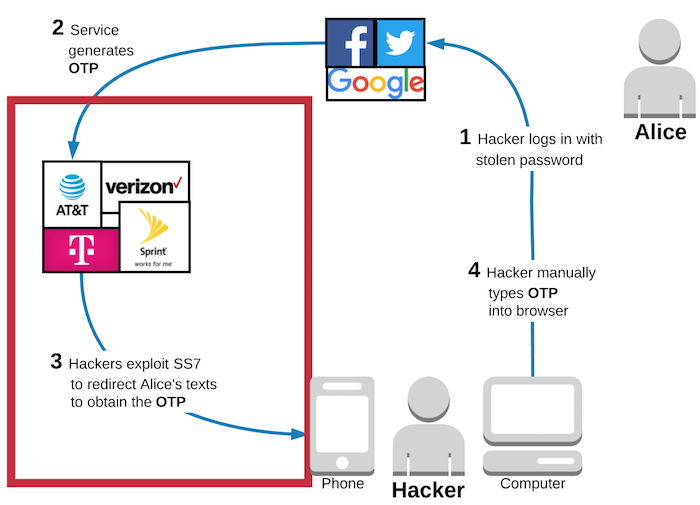
\includegraphics[width=10cm]{template/figures/SS7 attack vulnerable.png}
    \caption{SS7 haavoittuvuus SMS varmentamisessa \citep{2FA_SMS}}
    \label{fig:ss7SMSM}
\end{figure}

Vaikka SMS-varmenteeseen liittyy turvallisuusriski SS7 haavoittuvuuden takia on SMS-varmenteen käyttäminen suositeltavaa. NIST:in mukaan SMS-varmenteeseen liittyy turvallisuusongelmia, joista yksi on SS7 haavoittuvuus. NIST:in mukaan, vaikka SMS-varmenteeseen liittyy turvallisuusongelmia, on sen käyttäminen silti suositeltavaa. SMS-varmenteen käyttäminen parantaa turvallisuutta verrattuna yksivaiheiseen kirjautumineen. NIST kuitenkin toteaa, että SMS-varmenteen sijaan olisi suositeltavaa käyttää muita kirjautumismenetelmiä, jos mahdollista. Tulevaisuudessa NIST saattaa määritellä SMS-varmenteen huonoksi ja epäturvalliseksi vaihtoehdoksi \citep{NIST_800_63B}.



\section{TOTP}

Kuvassa \ref{fig:TOTP_service_provider} on merkattu punaisella ensimmäinen TOTP:n käyttämiseen liittyvä turvallisuusongelma. TOTP:n toiminta perustuu salaiseen avaimeen, jonka palvelun tarjoaja antaa käyttäjälle. Salainen avain näytetään yleensä QR-koodi muodossa, jonka pystyy skannaamaan puhelimella. Tähän liittyy turvallisuusriski. Jos hyökkääjä saa salaisen avaimen haltuunsa hänellä on pääsy TOTP:n kertakäyttöisiin koodeihin. Näin kaksivaiheisen kirjautumisen hyöty häviää.

\begin{figure}[ht]
    \centering
    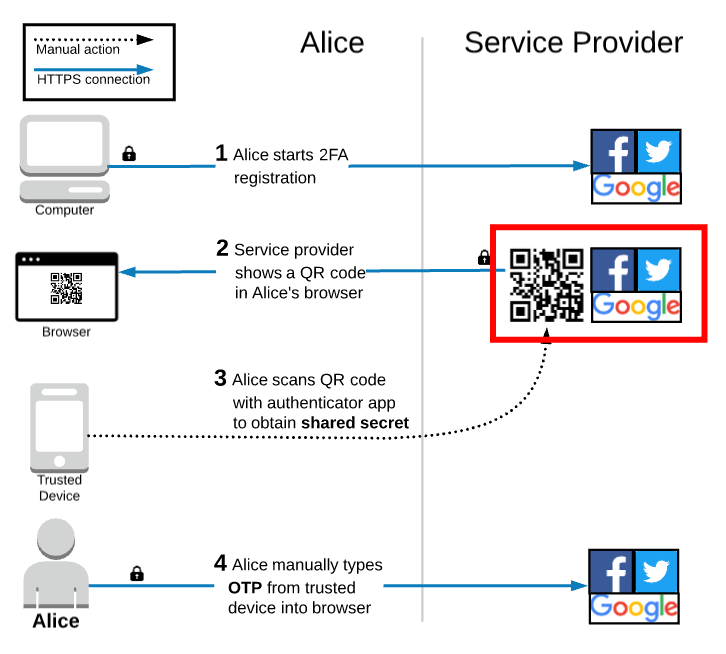
\includegraphics[width=10cm]{template/figures/TOTP service-provider-compromise.png}
    \caption{TOTP salaisen avaimeen turvallisuus ongelma \citep{TOTP}}
    \label{fig:TOTP_service_provider}
\end{figure}

\begin{figure}
    \centering
    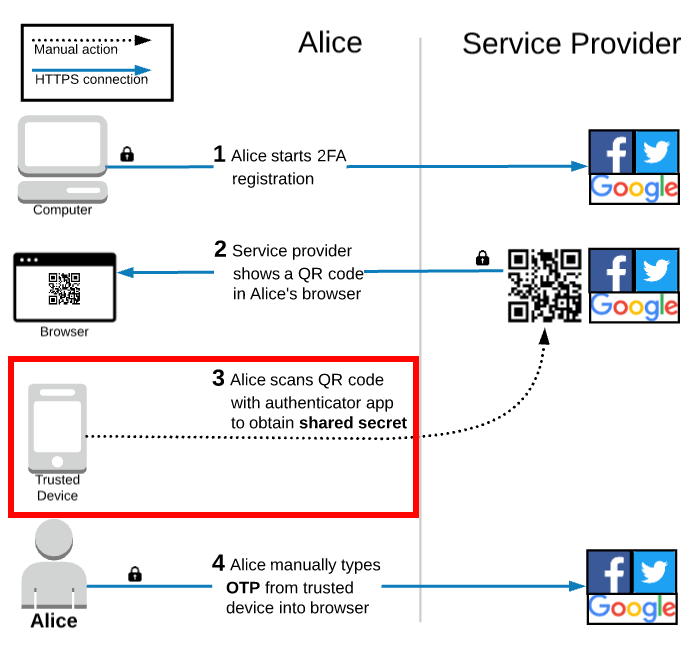
\includegraphics[width=10cm]{template/figures/TOTP trusted-device-compromise.png}
    \caption{TOTP luotetun laitteen turvallisuus ongelma \citep{TOTP}}
    \label{fig:TOTP_device}
\end{figure}

Kaksivaiheisessa kirjautumisessa, jossa käytetään TOTP:tä salaisten avaimien tallentamiseen käytetään yleensä luotettavana laiteena puhelinta. Puhelimeen on tallennettu salaiset avaimet, joiden perusteella kertakäyttöiset koodit luodaan. TOTP:n toinen turvallisuusriski liittyy puhelimeen. Kuvassa \ref{fig:TOTP_device} on punaisella merkitty tätä turvallisuusongelmaa. Puhelinta pidetään luotettuna laitteena ja oletetaan vain oikealla omistajalla olevan pääsy laitteelle. Puhelin voi hävitä tai se voidaan varastaa. Myös haittaohjelmat voivat varastaa TOTP salaiset avaimet.

Teknologien turvallisuus kehittyy ja paranee jatkuvasti. Yksi mittari on verkkosivujen siirtyminen käyttämään HTTPS-protokolaa. HTTPS-protokolan avulla verkkosivujen tiedot siirtyvät salatusti verkossa. Tällä hetkellä 95\% verkkosivuista käyttää HTTPS-protokollaa. Vaikka verkkosivujen turvallisuus on parantunut yksi asia, joka ei ole parantunut ja vähentynyt on kalasteluhyökkäykset \citep{google_transparency_report} \citep{phishing_scams}.

Kaksivaiheiseen tunnistautumiseen, jossa käytetään TOPT:tä liittyy kalasteluhyökkäyksen riski. Kalasteluhyökkäyksessä hyökkääjä on tehnyt aidon näköisen verkkosivun, jossa pyydetään käyttäjää antamaan käyttäjätietoja. Kalastelusivu voi olla aidon näköinen, joten käyttäjä luulee sivuston olevan aito ja oikea. Kuvassa \ref{fig:TOTP_phishing} on kuvattu kalastelusivun toimintaa. Ensimmäisessä ja kolmannessa kohdassa käyttäjä syöttää salasanan sekä kertakäyttöisen koodi. Käyttäjä luulee kirjautuvansa oikealle sivulle, mutta todellisuudessa käyttäjä syöttää tiedot kalastelusivulle. Kohdissa kaksi ja neljä hyökkääjä hyödyntää käyttäjän kalastelusivulla syöttämiä tietoja ja kirjautuu oikeaan palveluun. Näin hyökkääjä saa pääsyn käyttäjätilille. Vaikka kaksivaiheinen kirjautuminen oli käytössä ei se estä kalastelusivuihin liittyvää turvallisuusongelmaa.

\begin{figure}[ht]
    \centering
    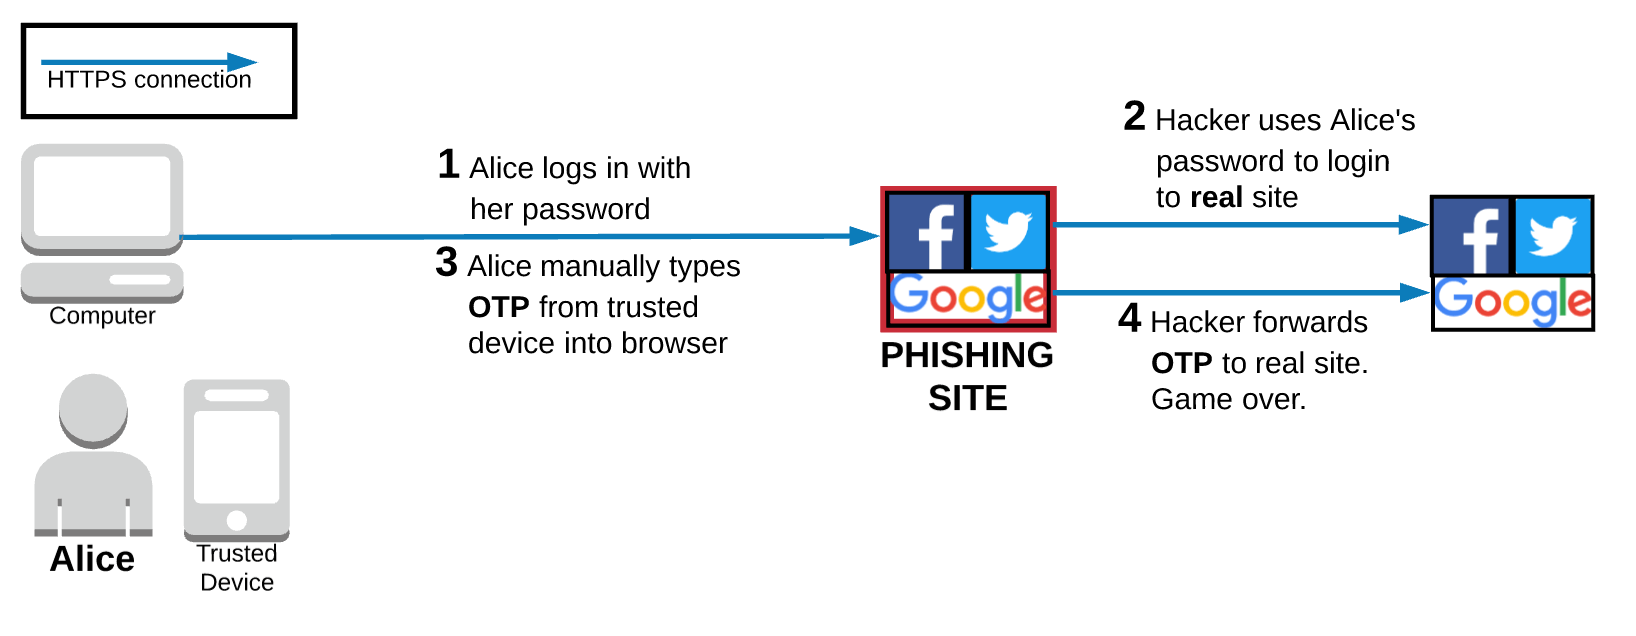
\includegraphics[width=15cm]{template/figures/totp phishing attack.png}
    \caption{TOTP kalasteluhyökkäys \citep{TOTP}}
    \label{fig:TOTP_phishing}
\end{figure}

Kuva \ref{fig:TOTP_phishing} kuvasi mahdollisen kalasteluhyökkäyksen toimintaa. Kalasteluhyökkäyksiä voidaan toteuttaa muillakin tavoilla. SMS-varmenne on myös haavoittuvainen kalasteluhyökkäykselle. SMS-varmentamisessa lähetetään kertakäyttöinen koodi tekstiviestinä käyttäjän puhelimeen. Hyökkääjä tarvitsee tämän koodin kirjautumista varten. Hyökkääjä voi yrittää kalastella tätä koodia lähettämällä käyttäjälle kalastelutekstiviestin, jossa pyydetään lähettämään äsken saatu kertakäyttöinen koodi \citep{google_transparency_report}.

Kalasteluhyökkäyksiä pyritään estämään monilla eri menetelmillä. Mobiilisovellukseen perustuva kaksivaiheinen kirjautuminen on parempi vaihtoehto. Se estää tekstiviesti- ja sähköposti kalasteluhyökkäyksiä, koska mobiilisovelluksella tapahtuvassa kirjautumisessa ei lähetetä tekstiviestiä tai sähköpostia.

Sähköpostissa tapahtuvia kalasteluhyökkäyksiä on mahdollista estää. Palveluntarjoajat voivat kehittää algoritmeja, jotka tunnistavat ja suodattavat mahdolliset kalasteluhyökkäysviestit. Automaattisten suodattimien lisäksi käyttäjä pystyy omalla toiminnallaan vaikuttamaan kalasteluhyökkäyksiin. Vaikka kalasteluhyökkäys on edelleen merkittävä ongelma nykyisillä sekä uusilla menetelmillä pyritään kalasteluhyökkäyksiä estämään \citep{google_transparency_report}.
